\documentclass{standalone}
\begin{document}
	\chapter{Vectors}
	\section{Definition}
	\quad A vector quantity is one which has magnitude and direction. For example, length is defined only by size and therefore is a \textit{scalar quantity}. However, acceleration due to gravity, while having a known magnitude, it is also acting in a particular direction. Hence, acceleration is a vector quantity.
	
	\begin{wrapfigure}{r}{0.25\textwidth}
		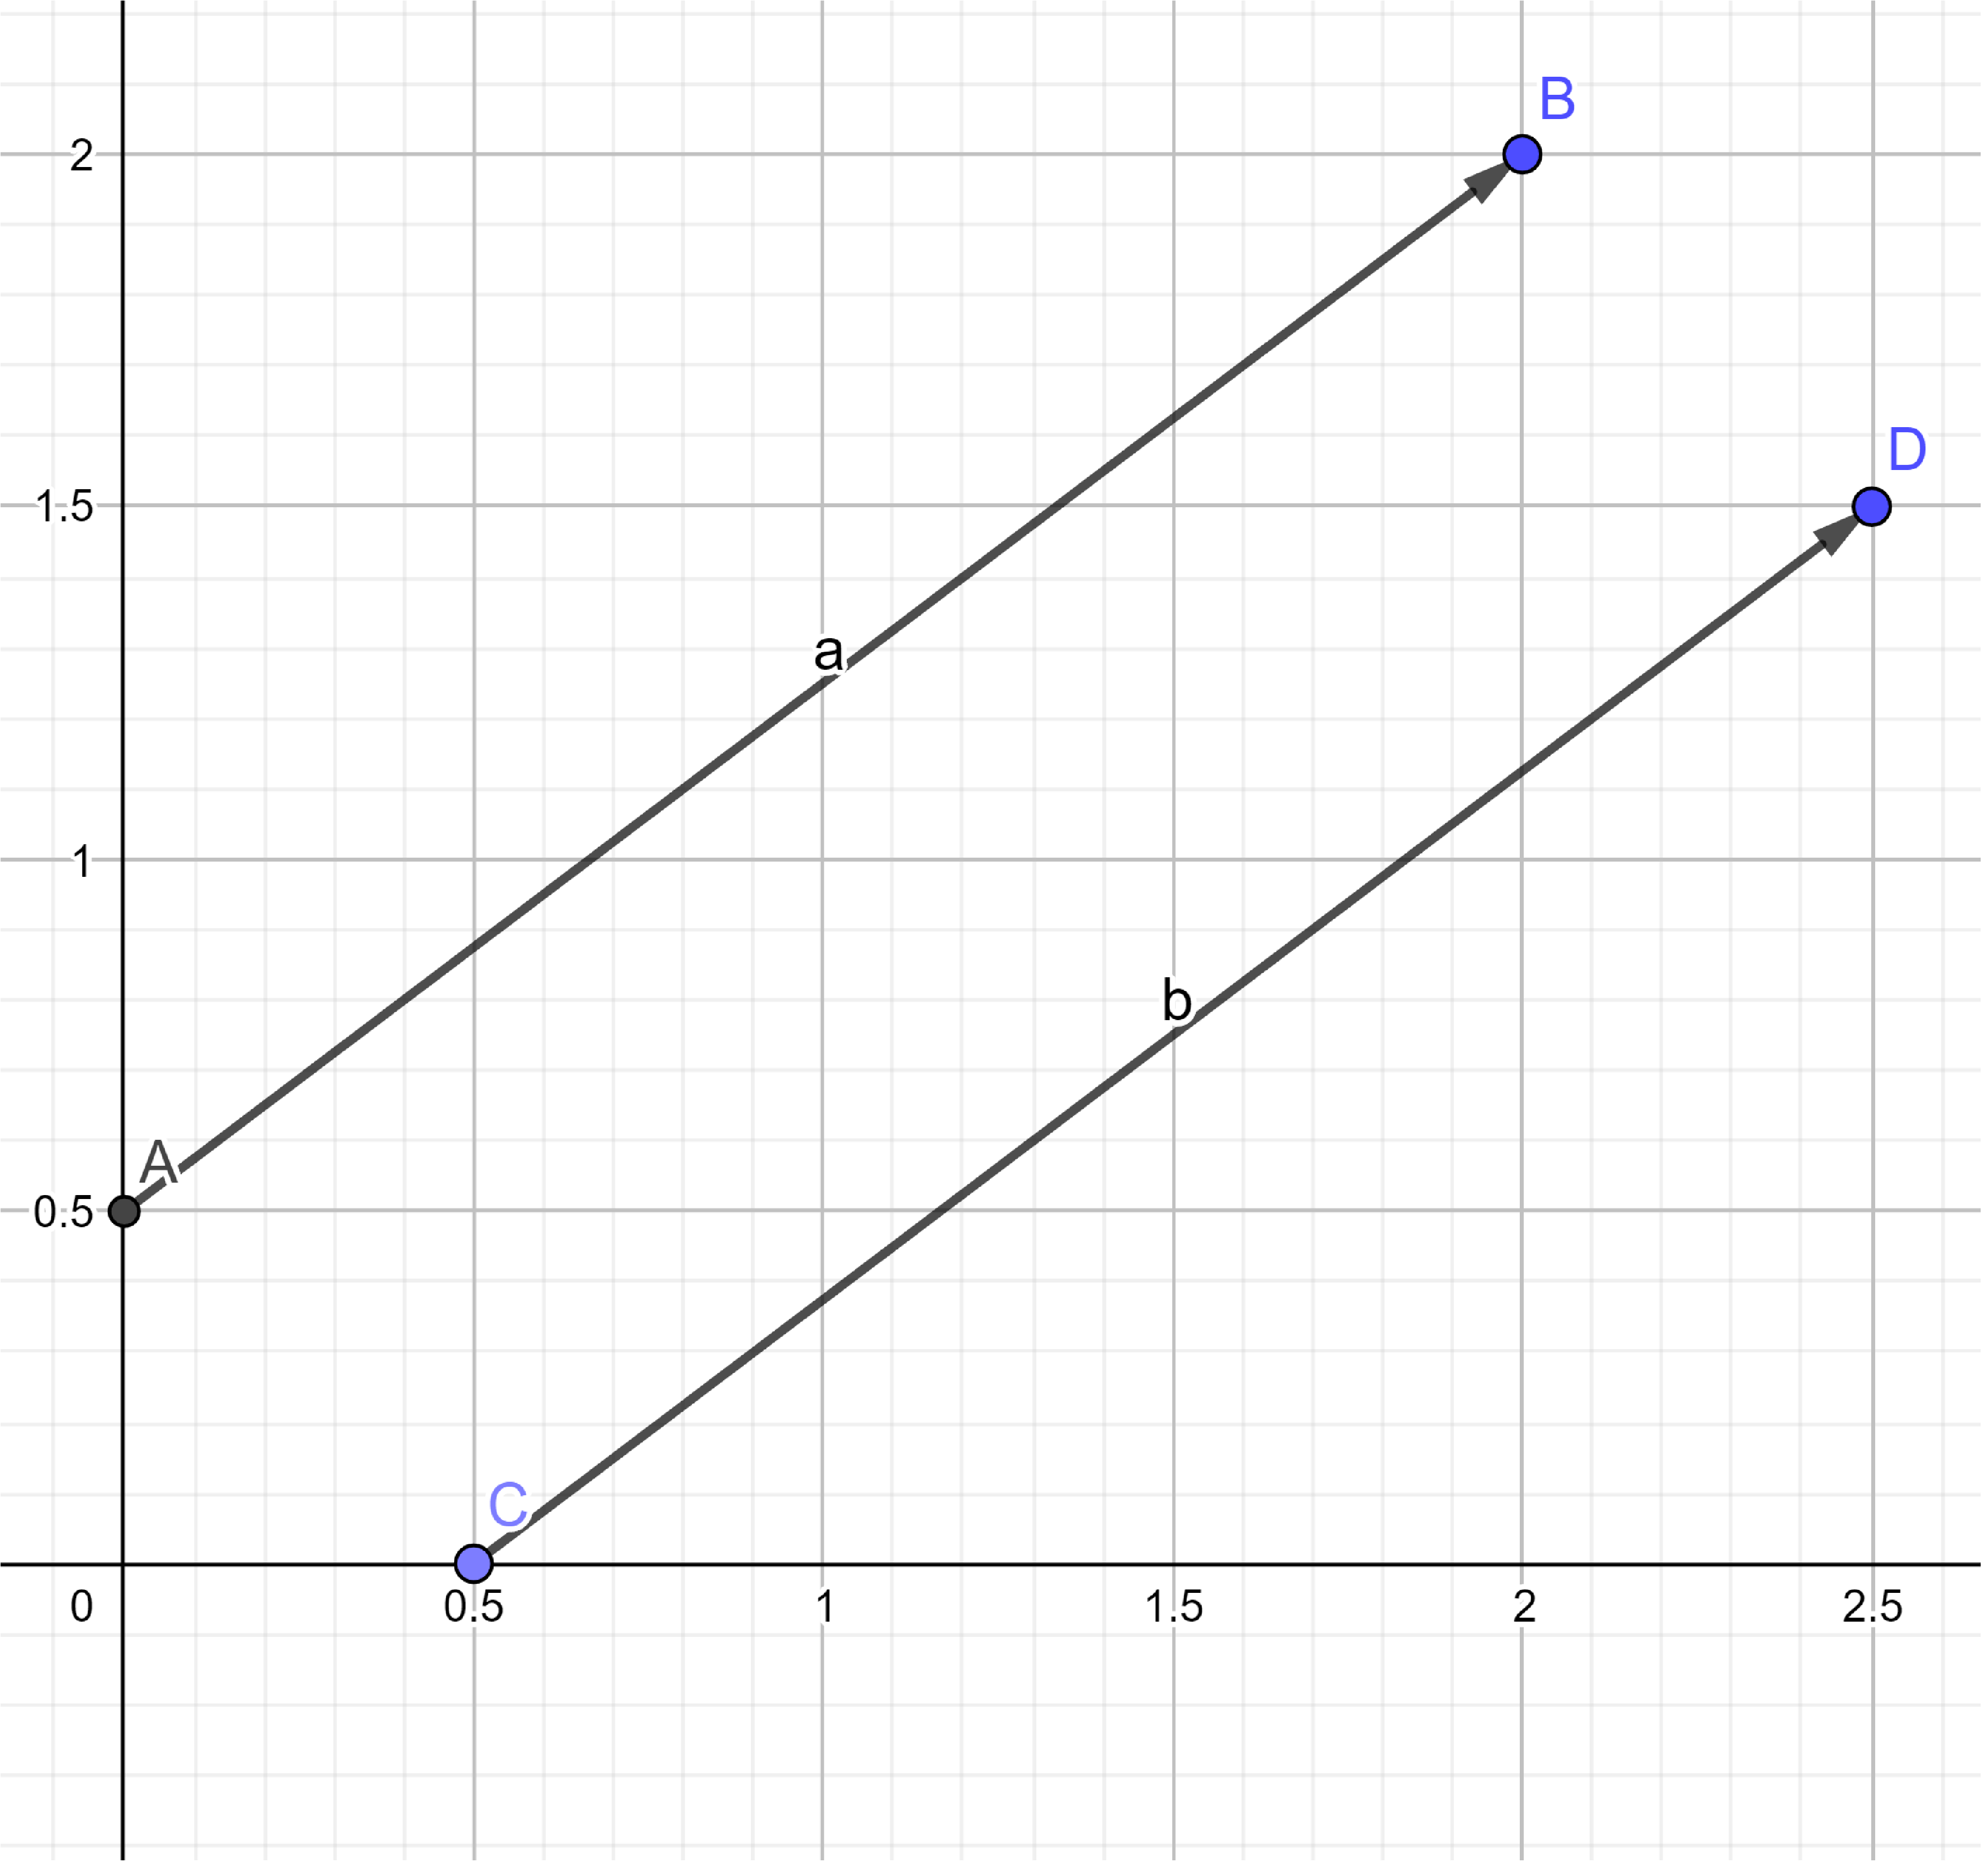
\includegraphics[width=1.3\linewidth]{vect_1} 
	\end{wrapfigure}
	
	Vectors are represented using line segments with arrows to denote their direction. Hence, we may consider vector $\overrightarrow{AB}$.
	
	\begin{itemize}
		\item{Two vectors are s.t.b equal iff they have the same magnitude and act in the same direction.}
		\item{The modulus refers to the size of a vector $\underline{a}$ and is denoted by $\abs{a}$.}
		\item{Two vectors $\underline{a}$ and  $-\underline{a}$  are equal in magnitude but opposite in direction. Hence the negative sign indicates opposing direction.}
		\item{When a vector is multiplied by a scalar, its magnitude changes. thus $\lambda  \underline{a}$ is a vector in the same direction as  $\underline{a}$ but has magnitude $\lambda\abs{\underline{a}}$}
	\end{itemize}
	\section{Position Vectors and Free Vectors}
	\quad When we refer to a vector  $\underline{a}$ we refer to a vector which is not confined to a specific position on the plane or in space.  $\underline{a}$, as such, is a \textit{free vector}.\\
	
	When we refer to the position vector  $\underline{b}$, we refer to a vector which is initially set to start from a specific location, usually, the origin.\\
	\setlength{\columnseprule}{0pt} 
	\begin{multicols}{2}
		\begin{center}
			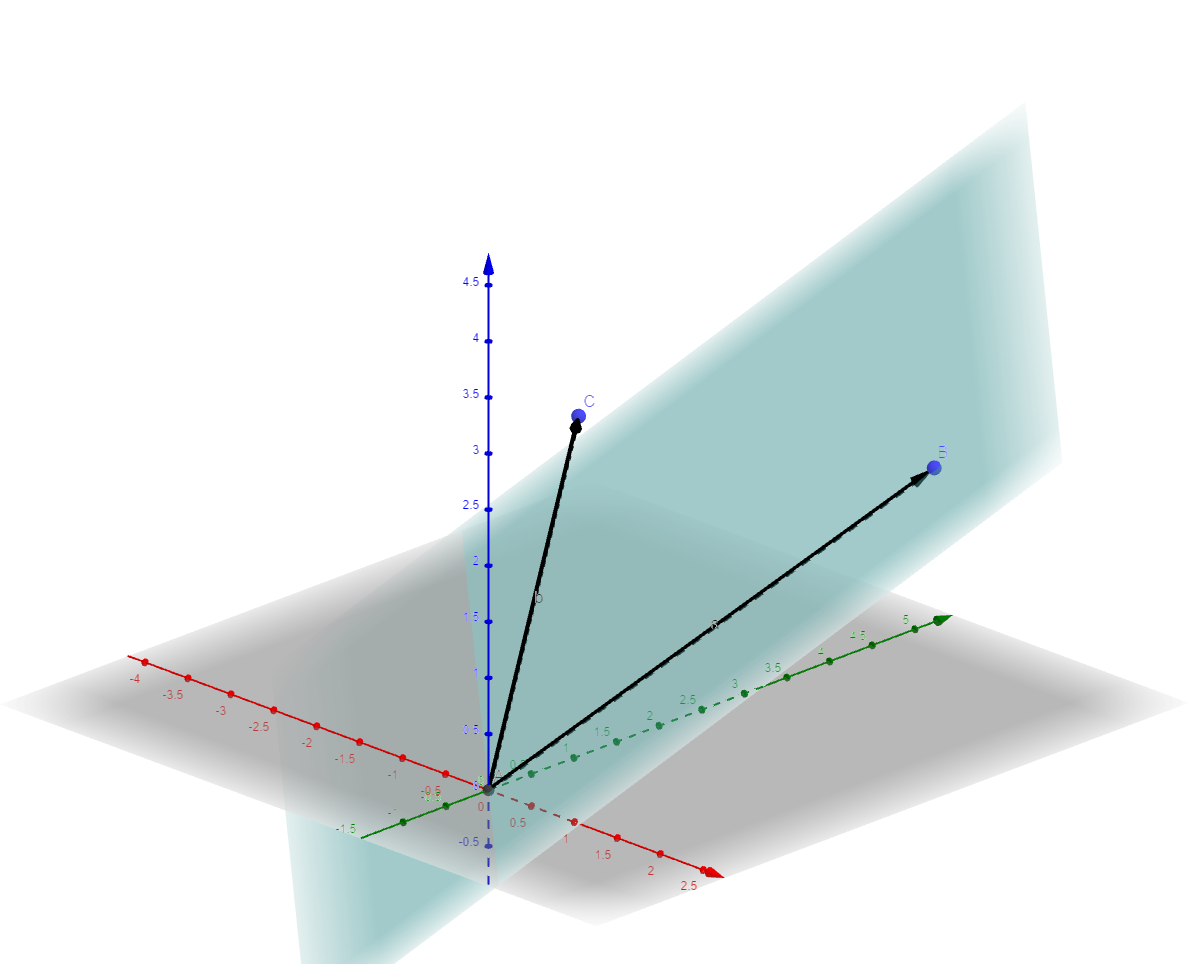
\includegraphics[scale=0.16]{vect_2} 
		\end{center}
		\begin{center}
			~\\~\\~\\
			Suppose that  $\underline{a}$ and  $\underline{b}$ are non-parallel free vectors, and that the origin is a fixed point. There exists only one plane which contains the point $(0,0)$,  $\underline{a}$ and  $\underline{b}$.
		\end{center}
		
	\end{multicols}
	
	Consider another point $p$ on this plane.
	\begin{multicols}{2}
		\begin{center}
			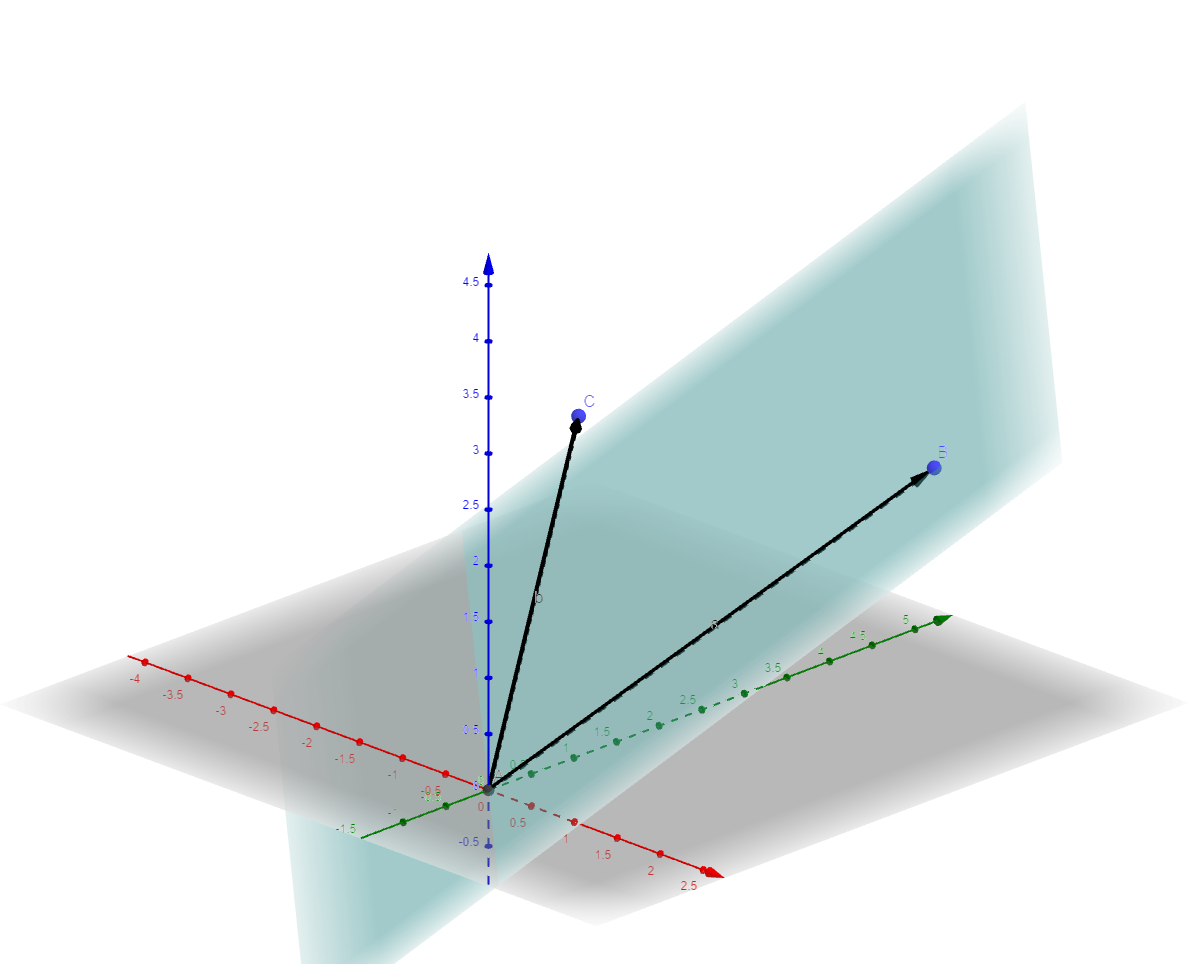
\includegraphics[scale=0.16]{vect_2} 
		\end{center}
		\begin{itemize}
			\item{$\vec{OP}$ is the PV \footnote{Position Vector} of P}
			
			\item{	$\overrightarrow{OC}$ is $\parallel$ to $\textbf{b}$, thus $\overrightarrow{OC} = \lambda \textbf{b}$}
			\item{$\overrightarrow{CP}$ is $\parallel$ to \textbf{a}, thus $\overrightarrow{CP} = \gamma \textbf{a}$}
			\item{$\overrightarrow{OP} = \overrightarrow{OC} + \overrightarrow{PC}	 =\gamma \textbf{a} + \lambda \textbf{b}$}
		\end{itemize}
		
	\end{multicols}
	~\\
	
	Therefore, the point $O$ and the vectors \textbf{a} and \textbf{b} form a frame of reference for the position of any point on the plane. The vectors \textbf{a} and \textbf{b} are known as the base vectors. Any vector parallel to the plane can be expressed in the form $\gamma \textbf{a} + \lambda \textbf{b}$ where $\lambda$ and $\gamma$ are scalar quantities.\\
	
	
	This basis spans the usual $x$ and $y$ plane. The base vectors are \textbf{i} and \textbf{j} respectively denoting the unit base vector in the positive $x$ direction and similarly in the positive $y$ direction.\\
	
	In general, given the points $A(x_1,y_1)$ and $B(x_2,y_2)$, the vector $\overrightarrow{AB}$ is given by:	
	
	
	\begin{center}
		\begin{tcolorbox}[center title,hbox,    %%<<---- here
			lifted shadow={1mm}{-2mm}{3mm}{0.1mm}%
			{black!50!white}]
			\begin{varwidth}{\textwidth}
				\begin{center}
					$$\overrightarrow{AB} = (x_2 -x_1)\textbf{i} - (y_2 -y_1)\textbf{j}$$
					
					$$	\abs{\overrightarrow{AB}} = \sqrt{(x_2 -x_1)^2 + (y_2 -y_1)^2}$$
				\end{center}
			\end{varwidth}
		\end{tcolorbox} 
	\end{center}
	\newpage
	\section{Unit vectors}
	
	
	
	A unit vector is a vector with magnitude 1. Consider vector $\textbf{v}$ \& let $\abs{\textbf{v}}$ be its magnitude. A unit vector in the direction of $\textbf{v}$, denoted by $\hat{\textbf{v}}$ can be obtained by dividing $\textbf{v}$ by its magnitude.
	
	$$\hat{\textbf{v}} = \frac{\textbf{v}}{\abs{\textbf{v}}}$$
	
	
	\section{Vectors in 3D space}
	
	The ideas developed in the previous section can be extended to the 3-dimensional space. Thus any point $A(x_1,y_1,z_1)$ in the 3D space has position vector $\overrightarrow{OA}$.
	\begin{center}
		\begin{tcolorbox}[center title,hbox,    %%<<---- here
			lifted shadow={1mm}{-2mm}{3mm}{0.1mm}%
			{black!50!white}]
			\begin{varwidth}{\textwidth}
				\begin{center}
					$$\overrightarrow{OA} = x\textbf{i} + y\textbf{j} +z\textbf{k}$$
					$$\abs{\overrightarrow{OA} = \sqrt{x^2 + y^2 + z^2}}$$
				\end{center}
			\end{varwidth}
		\end{tcolorbox} 
	\end{center}
	
	Also, given two points $A(x_1,y_1,z_1)$ and $B(x_2,y_2,z_2)$, the vector $\overrightarrow{AB}$ is given by:
	\begin{center}
		\begin{tcolorbox}[center title,hbox,    %%<<---- here
			lifted shadow={1mm}{-2mm}{3mm}{0.1mm}%
			{black!50!white}]
			\begin{varwidth}{\textwidth}
				\begin{center}
					$$\overrightarrow{AB} = (x_2 -x_1)\textbf{i} - (y_2 -y_1)\textbf{j} + (z_2 - z_1)\textbf{k}$$
					
					$$	\abs{\overrightarrow{AB}} = \sqrt{(x_2 -x_1)^2 + (y_2 -y_1)^2 + (z_2 - z_1)^2}$$
				\end{center}
			\end{varwidth}
		\end{tcolorbox} 
	\end{center}
	
	\subsection{Direction ratios of a Vector}
	
	Given the vector $a\textbf{i}+b\textbf{j}+c\textbf{k}$, the ratios $a\colon b\colon c$ are called the direction ratios of the vector.\\
	
	Since the numbers $a$, $b$ and $c$ define the inclination of the vector in space, it follows that parallel vectors have equivalent direction vectors.\\
	
	In vectors, parallelism can be of two types:\\
	\begin{itemize}
		\item{Like parallel}
		\subitem{Two like parallel vectors both travel in the same direction.}
		\item{Unlike parallel}
		\subitem{Two unlike parallel vectors are still positionally parallel but act in the opposite direction.}
	\end{itemize}
	~\\
	In both cases, the direction ratios, however, are the same. For instance, consider the two vectors:
	
	\begin{alignat*}{2}
		&   & \textbf{a} & = 3\textbf{i} + 5\textbf{j} + 6\textbf{k}  \\
		&   & \textbf{b} & = -3\textbf{i} -5\textbf{j}  - 6\textbf{k} 
	\end{alignat*}
	Both of them will simplify to an equivalent ratio when multiplied by $-1$.
	
	\subsection{3-Dimensional Lines}
	
	Lines in 3D are better explained through vector geometry. Coordinate geometry is sufficient for the analysis of lines in 2D, however, when adding the third dimension, this becomes inefficient.
	
	\subsubsection{Equation of a straight line}
	
	The previous notion of the definition of a straight line, $y=mx+c$ or more particularly $y_2-y_1 = m(x_2-x_1)$ becomes insufficient to define a line on 3 planes of space.\\
	
	A line in 3D space is defined by a point through which it passes, and a direction to which it is parallel. Consider the following diagram:
	
	
	\begin{center}
		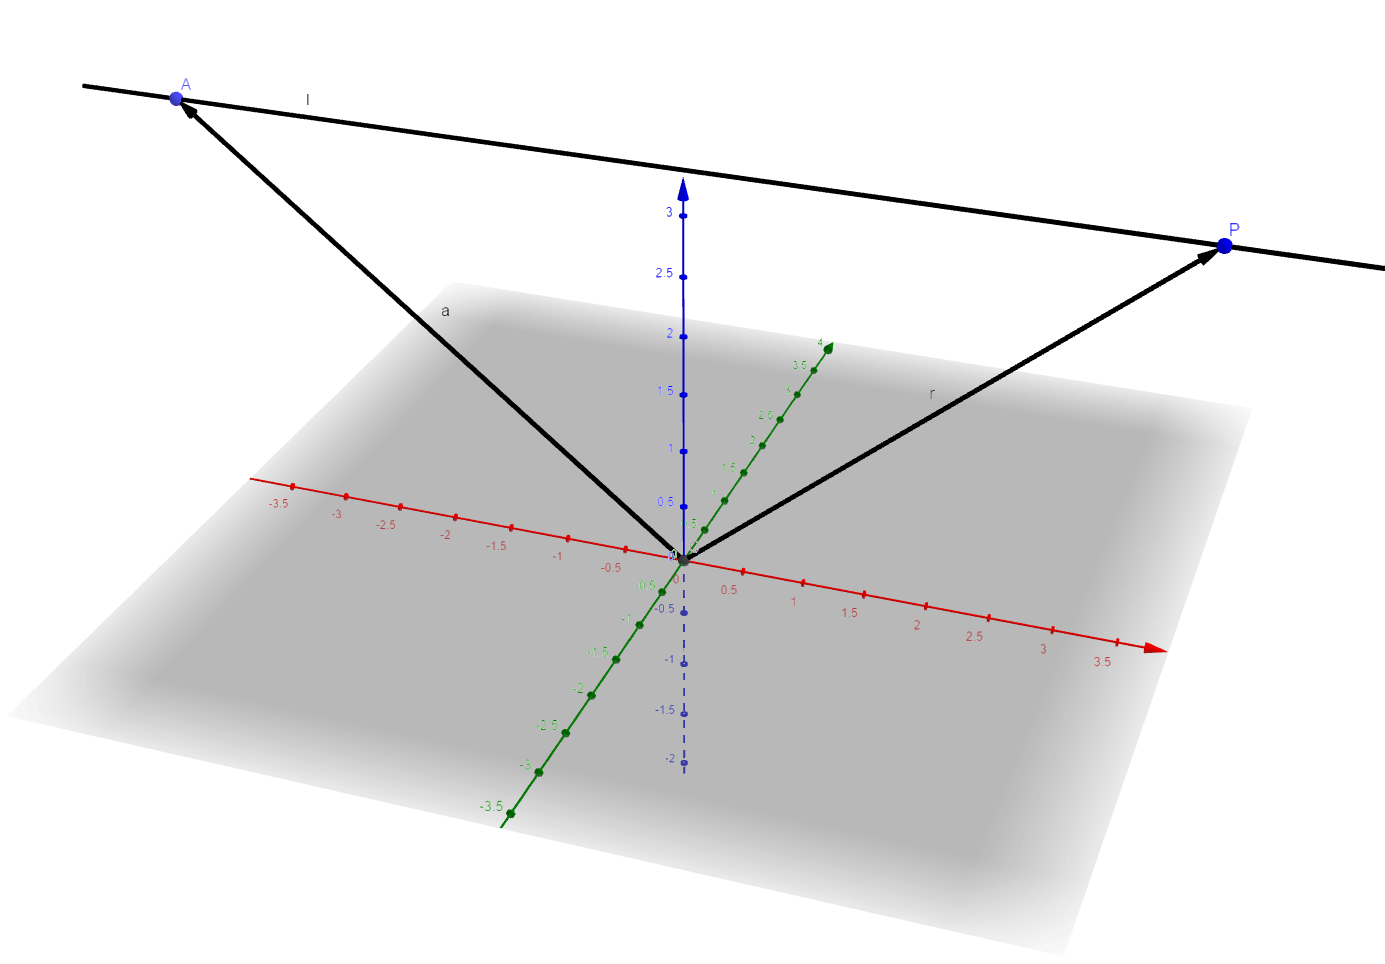
\includegraphics[scale=0.15]{vect_3}
	\end{center}
	
	
	Let $A$ be a fixed point on the line $l$ with position vector $\textbf{a}$ \& let $P$ represent a general point on the line. Let the position vector of $P$ be $\textbf{r}$. Consider also a vector $\textbf{m}$ parallel to the line $l$.\\
	
	We need to find the equation of line $l$, specifically, a rule defining the line $l$ which governs all points $P$ on this line. To generate the line $l$ as described above, the point $P$ must be such that $\overrightarrow{AP}$ is parallel to $\textbf{m}$.
	
	\begin{multicols}{3}
		$$	 \textbf{r}  = \textbf{a} + \lambda \textbf{m}$$
		
		\begin{alignat*}{2}
			&   & x & = x_1 + \lambda a \\
			&   & y & = y_1 + \lambda b \\
			&   & z & = z_1 + \lambda c 
		\end{alignat*}
		\begin{alignat*}{2}
			&   & x & = x_1 + \lambda a \\
			&   & y & = y_1 + \lambda b \\
			&   & z & = z_1 + \lambda c 
		\end{alignat*}
		\begin{center}
			~\\
			~\\
			$\frac{x-x_1}{a} = \frac{y-y_1}{b} = \frac{z-z_1}{c}$
		\end{center}
	\end{multicols}
	\end{document}